\documentclass[conference]{IEEEtran}


\usepackage{cite}
\usepackage{amsmath,amsfonts}
\usepackage{amssymb}
\usepackage{graphicx}
\usepackage{url}
\usepackage{booktabs}
\usepackage{array}

\usepackage{tikz}
\usetikzlibrary{shapes.geometric, arrows.meta, positioning}

\makeatletter
\renewcommand{\subsection}{%
    \@startsection{subsection}{2}{\z@}%
    {2.5ex plus 1ex minus 0.2ex}%
    {1.0ex plus 0.2ex}%
    {\normalfont\normalsize\bfseries}%
}
\makeatother

\makeatletter
\renewcommand{\subsubsection}{%
    \@startsection{subsubsection}{3}{\z@}%
    {1.5ex plus 0.5ex minus 0.2ex}%
    {0.8ex plus 0.2ex}%
    {\normalfont\normalsize}%
}
\makeatother


\title{Design and Implementation of a 5-DOF Pick and Place Robotic Arm
}


\author{
    \IEEEauthorblockN{
        Abeywardhana S D,
        Chamodya B J,
        Hettiarachchi S M
    }
    \IEEEauthorblockA{
        Department of Computer Engineering\\
        Faculty of Engineering\\
        University of Sri Jayewardenepura\\
        Sri Lanka
    }
}

\begin{document}

\maketitle

\begin{abstract}
Automation of object handling tasks is a significant technological advancement in most of the modern world applications. This project carefully examines the design and the development of a five-degree-of-freedom (5 DOF) robotic arm which is specifically designed for automated pick-and-place operations. The main movements of the robotic arm is determined using inverse kinematics which is a mathematical process commonly used to calculate the required rotation angles of each joint based on the desired position of the end effector. The object detection system has been implemented to identify the target object and coordinate-based positioning is combined to achieve the required movements during this whole process. Mechanical and electronic simulations were also integrated and the system’s future implementations will develop this system further. This research is mainly focused on the integration of robotic kinematics, mechanical design and embedded control of the robotic arm.


\end{abstract}


\begin{IEEEkeywords}
Robotic arm, 5 DOF, Kinematics, Mechanical structure , Pick-and-place, Electronic system, Micro-controller, Object detection, Challenges and implementation

\end{IEEEkeywords}


\section{Introduction}

Robotics is an important section of engineering which focuses on the design, development and control of machines capable of performing tasks autonomously. Robots are commonly being used in modern applications that can replace humans in a number of occupations by their own structures and operations. Especially industrial robotic designs, they combine mechanical structures, electronic components, sensors, actuators and other computational techniques and are used for the industrial tasks like transporting and unloading materials, assembling, measuring, etc. Therefore, the demand for this kind of robotic designs is gradually increasing and manufacturing of the types of robots are increasing with higher precision and greater productivity. 

Robotic arms are one of the robotic systems that are widely used for material handling, assembly, manufacturing and pick-and-place operations in various industries. It functions more similarly to a human arm. A robotic arm consists of connected links, joints and gripper mechanism which provide movement and pick-and-place operations within the defined workspace.  In robotics, Degree Of Freedom (DOF) is defined as the number of independent axes that a robot can move. In most of the manufacturing industry, robotic arms have replaced human hands with applications like assembling, repairing and pick-and-place goods according to their assigned placements. 
As mentioned before, pick-and-place is one of the fundamental applications of robotic arms in industry where an object is picked from one location and transferred to another. All joints of the robotic arm should be accurately positioned for this task to succeed. The accurate joint configurations and the coordinate system is calculated by using inverse kinematics. Inverse kinematics establishes the relationship between the desired position of the end effector and the corresponding joint angles of the robotic arm. 

The purpose of this project is focused on the design and implementation of the 5 DOF robotic arm with the goal of performing an automated pick-and-place operation. This system integrates mechanical structure which designed using SolidWorks, servo motors, ESP32 microcontroller and a gripper mechanism Considering the structure of this paper, literature review, system overview and architecture, mechanical design and prototype development, Inverse kinematics model and angle calculation , electronic system and microcontroller implementation, experimental results and discussion and finally future improvements and the references. 


\section{literature review}

Pick and place requirement is one of the common applications of robotics in modern industries. Research has demonstrated robotic arms which are capable of detecting, grasping and transferring the objects between two different locations. One of the examples is an intelligent six-axis robotic arm which used for pick-and-place operations which is used for object recognition and demonstrated the integration of object detection with robotic manipulation.\cite{tung2023}

The kinematics are the main concept of the robotic arm control; it ensures the movements of the end effector and according to that the configuration of the individual joints in the system. Inverse kinematics is used to determine the joints’ angles and other variables to position the end effector at the target location accurately. This concepts investigates both analytical and learning based approaches and analytical methods providing solutions based on the mathematical model of the robotic manipulator.\cite{wagaa2023}

Automated pick-and-place systems consist of various units and object detection is one of the important ones. It should identify the object correctly and determine when and where the object is available for manipulation. Previous research has investigated camera-based object detection and machine-learning approaches. Specially vision-based systems are developed for this purpose in most modern robotic systems and provide the coordinates to the robotic arm for the pick-and-place operations. \cite{kumar2014}

Most robotic designs are integration of object detection, kinematic computation, actuator control within embedded platforms etc. A recent six DOF robotic arm study which integrated object detection and robot control on a resource constrained microcontroller is one of the examples for the demonstration of the possibility of performing perception and manipulation using an embedded architecture.\cite{almaliki2026}


\section{system overview and architecture}

The project is a five-degree-of-freedom (5-DOF) robotic arm that integrates a mechanical robotic arm structure, servo motors, an ESP32 microcontroller, a gripper mechanism and an object detection system using sensors. These components work together and the main process  is to identify the target object, determine its position, move the robotic arm to the required location, pick the object and place it inside a designated container. The overall system combines mechanical design, embedded control and inverse kinematics concepts to achieve the required pick-and-place operation. 

\subsection{System Overview}

This robotic arm is a 5 DOF system which consists of five joints and two links and end effector.  Servo motors are used to control each joint movement and the end effector (gripper) reaches the required position to pick and place the objects within the defined workspace. The gripper mechanism is used to grasp and release the object from one place to another.

The main control unit of this robotic arm is the ESP32 microcontroller. The main purpose of it is to gather the required movement information  of the five joints and generate the control signals for the servo motors and control the all joints of the robotic arm and the gripper mechanism.  
 
The object detection in this robotic design is mainly done by the IR sensor. It identifies the arrival of the object to the defined position and  according to that it determines the information required for the pick-and-place operation. The information which gets by the IR sensor will be provided to the control system. After getting this information about the object, the required joint angles using inverse kinematics based on the position of the end effector. 

\subsection{System Architecture}

The overall system architecture of this robotic arm includes a few main units such as ESP32 microcontroller, servo motors and control system, IR sensor and the object detection system and the arm structure. All these units are interconnected together and work as a complete system that can perform required pick-and-place operation. 


\begin{figure}[htbp]
    \centering

    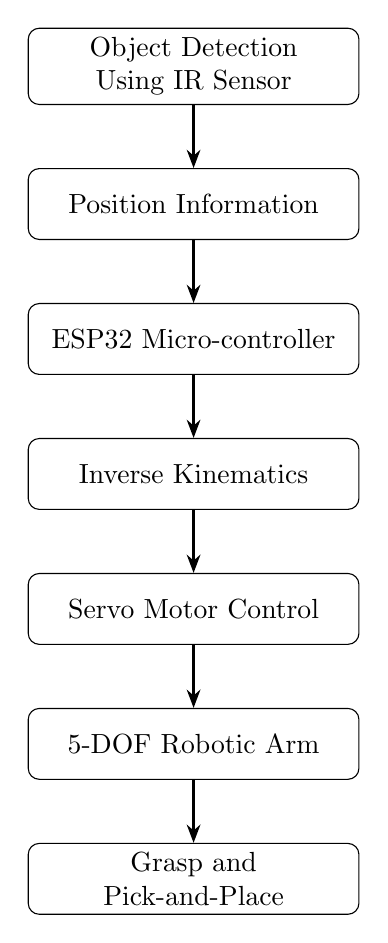
\begin{tikzpicture}[
        node distance=8mm,
        box/.style={
            rectangle,
            draw,
            rounded corners,
            minimum width=42mm,
            minimum height=9mm,
            align=center
        },
        arrow/.style={
            -{Stealth},
            thick
        }
    ]

    \node[box] (sensor) {Object Detection\\Using IR Sensor};

    \node[box, below=of sensor] (position) {Position Information};

    \node[box, below=of position] (esp32) {ESP32 Micro-controller};

    \node[box, below=of esp32] (ik) {Inverse Kinematics};

    \node[box, below=of ik] (servo) {Servo Motor Control};

    \node[box, below=of servo] (arm) {5-DOF Robotic Arm};

    \node[box, below=of arm] (operation) {Grasp and\\Pick-and-Place};

    \draw[arrow] (sensor) -- (position);
    \draw[arrow] (position) -- (esp32);
    \draw[arrow] (esp32) -- (ik);
    \draw[arrow] (ik) -- (servo);
    \draw[arrow] (servo) -- (arm);
    \draw[arrow] (arm) -- (operation);

    \end{tikzpicture}

    \caption{Overall system flow of the proposed pick-and-place robotic arm}
    \label{fig:system_flow}

\end{figure}

\begin{figure}[htbp]
    \centering
    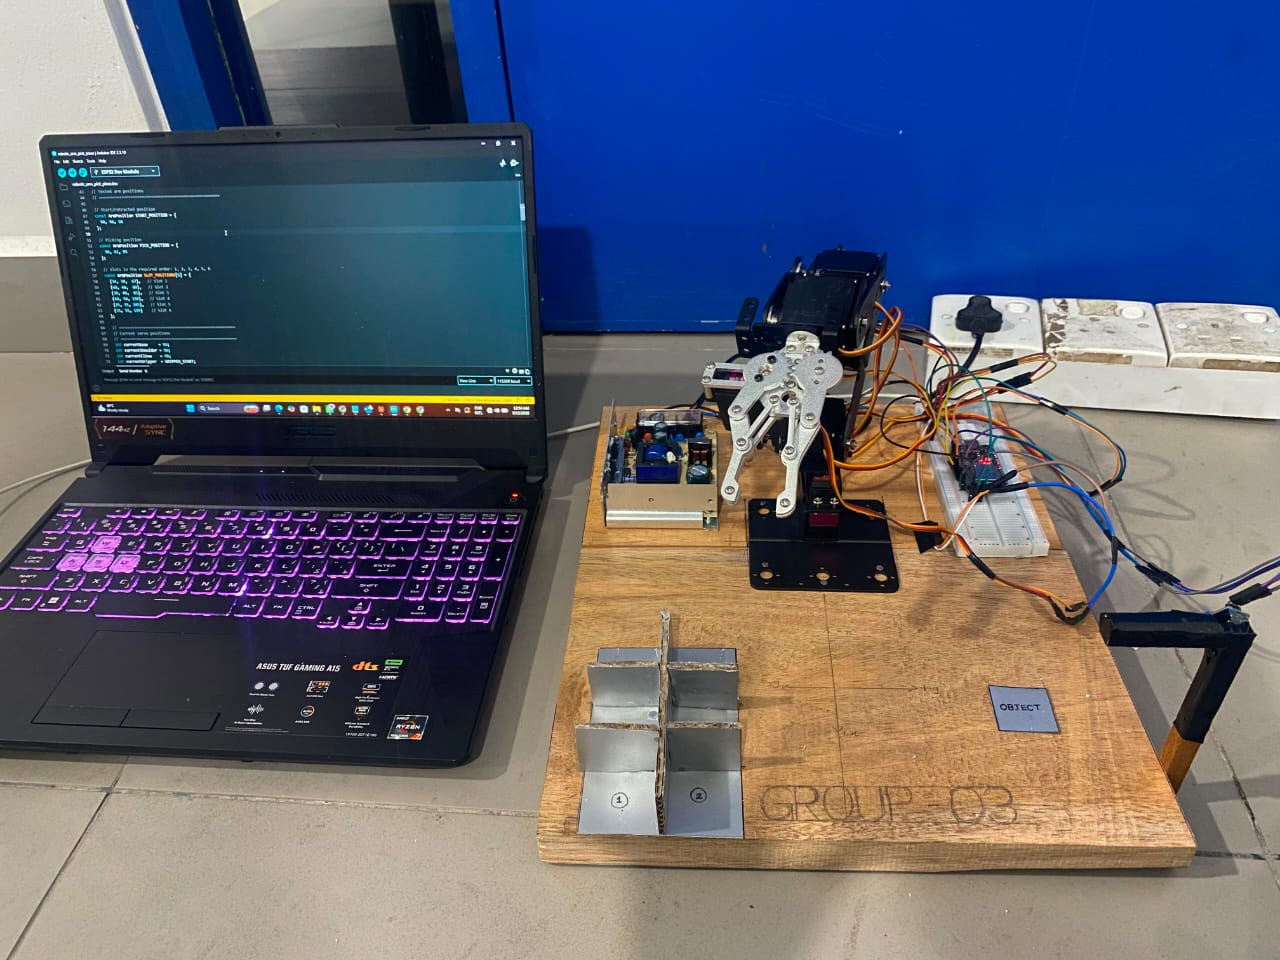
\includegraphics[width=\columnwidth]{figures/system architecture.jpeg}
    \caption{Overall system architecture of the 5-DOF pick-and-place robotic arm}
    \label{fig:system architecture}
\end{figure}


\subsection{Working Principle}

The working process of the proposed system consists of several stages. As the first step the ESP32 and the connected servo motors are initialized. The initial position of the robotic arm is predefined and the required system parameters such as angles of each joint are loaded before starting the operation.

The object detection is done by using an IR sensor at the predefined detection position. The main process is identifying the object by emitting infrared radiation and detecting the reflected signal from the object. When an object is detected by the sensor within the sensing range, it provides a corresponding signal to the ESP32 and this signal initiates the required pick-and-place operation. 

Inverse kinematics is used to calculate the joint angles based on the desired position of the robotic arm. After object detection, the control algorithm determines the joint configurations and ESP32 sends the control signals to the servo motors to move correctly toward the calculated pick position. 

When the end effector reaches the required object picking position which is calculated before, the gripper is activated and grasps the target object. After the object grasp, the gripper remains closed until the object is in the correct position. The gripper will securely hold the object while the robotic arm moves toward the target position and then releases the object.

After successfully picking the object the arm will move to the predefined target location which is determined using inverse kinematics calculations. The servo motors are controlled according to the joint angles and required joint configuration to place the object in the correct place by positioning the end effector correctly. 

The gripper opens to release the object when the end effector reaches the target location correctly. After releasing the object in the correct position, the robotic arm returns into the predefined initial position for the next pick-and-place process. 


\section{mechanical design and prototype development}

The robotic arm is designed with 5 DOF that has a working dimension which is similar to a human arm and it is capable of grasping an object along a predefined trajectory. The mechanical design of it was considered to develop a suitable structure capable of performing the pick-and-place operation. The design process initially focused on determining the required degrees of freedom, joint movements, workspace and arrangement of the robotic arm links. 

\subsection{Mechanical Design Concept}

The main mechanical design concept is focused on five degrees of freedom that allow the arm to perform coordinated movements through its different joints and position the end effector at the required locations within its intended workspace. The lengths and orientations of the links were determined according to the required movements to provide sufficient reach for the intended pick-and-place task. 

\subsection{SolidWorks CAD Modeling}

The three-dimensional CAD model of this robotic arm was developed using SolidWorks 2022 software. All mechanical components and parts were designed individually and then combined them to form the complete robotic arm assembly. All these links, joints and the structure were designed according to the predefined dimensions and mechanical constraints which were required for the desired application. This model provides a visual representation of the proposed mechanical structure. It was used to support the evaluation of the initial design before going to the physical prototype.

\begin{figure}[htbp]
    \centering
    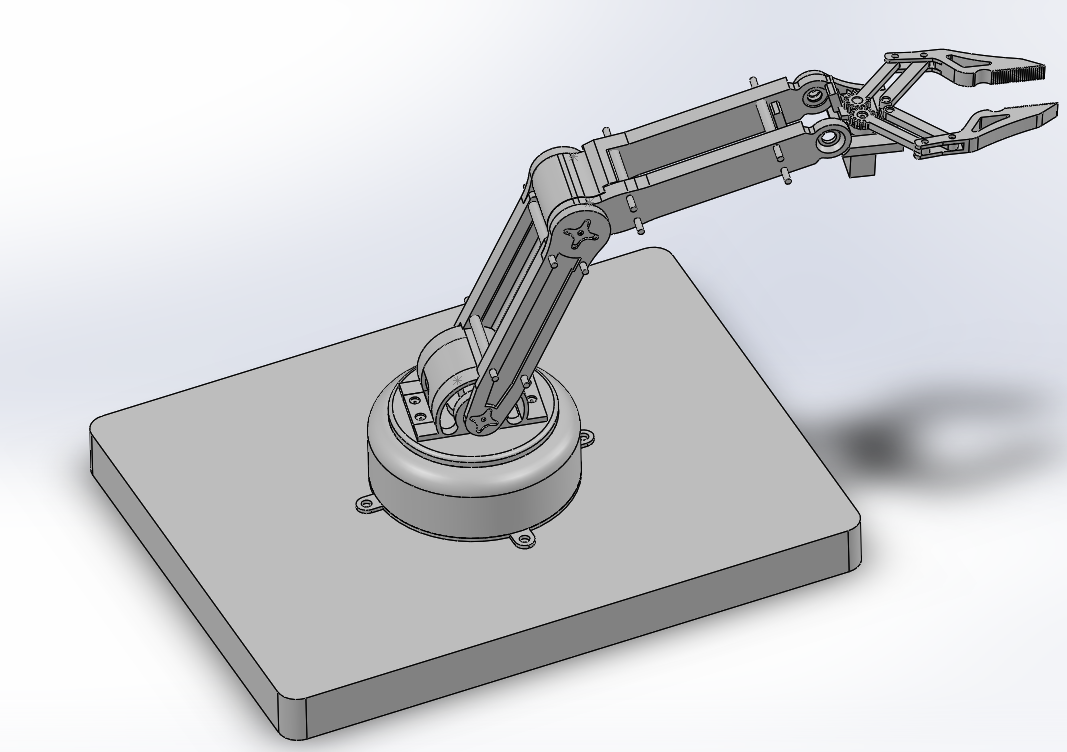
\includegraphics[width=\columnwidth]{figures/solidworks design.png}
    \caption{3D model of the proposed 5-DOF robotic arm}
    \label{fig:Solid design}
\end{figure}

\subsection{Final Prototype Structure Selection}

A metal robotic arm structure was used for the final prototype due to the practical requirements of fabrication and implementation of the initial robotic arm structure which was designed using SolidWorks. This arm structure was selected to reduce fabrication complexity, accelerate the implementation process and increase the reliability of the system. It was adapted to accommodate the required servo motors, gripper mechanism and object detection sensor which maintains the required five-degree-of-freedom configuration.  

\subsection{Final Mechanical Assembly}

The final mechanical assembly of this system consists, arm structure, servo motors, gripper mechanism and sensor mounting arrangement. Each servo motor is installed at the corresponding joints to provide controlled movement of the structure during the pick-and-place operation. Gripper mechanism is used for grasping and releasing the object in the right positions and it is mounted at the end effector. The sensor mounting system was designed to correctly detect the object while avoiding interference with the movement of the robotic arm. This final mechanical assembly was checked to ensure that the robotic arm could perform the required movements for the pick-and-place operation.

\begin{figure}[htbp]
    \centering
    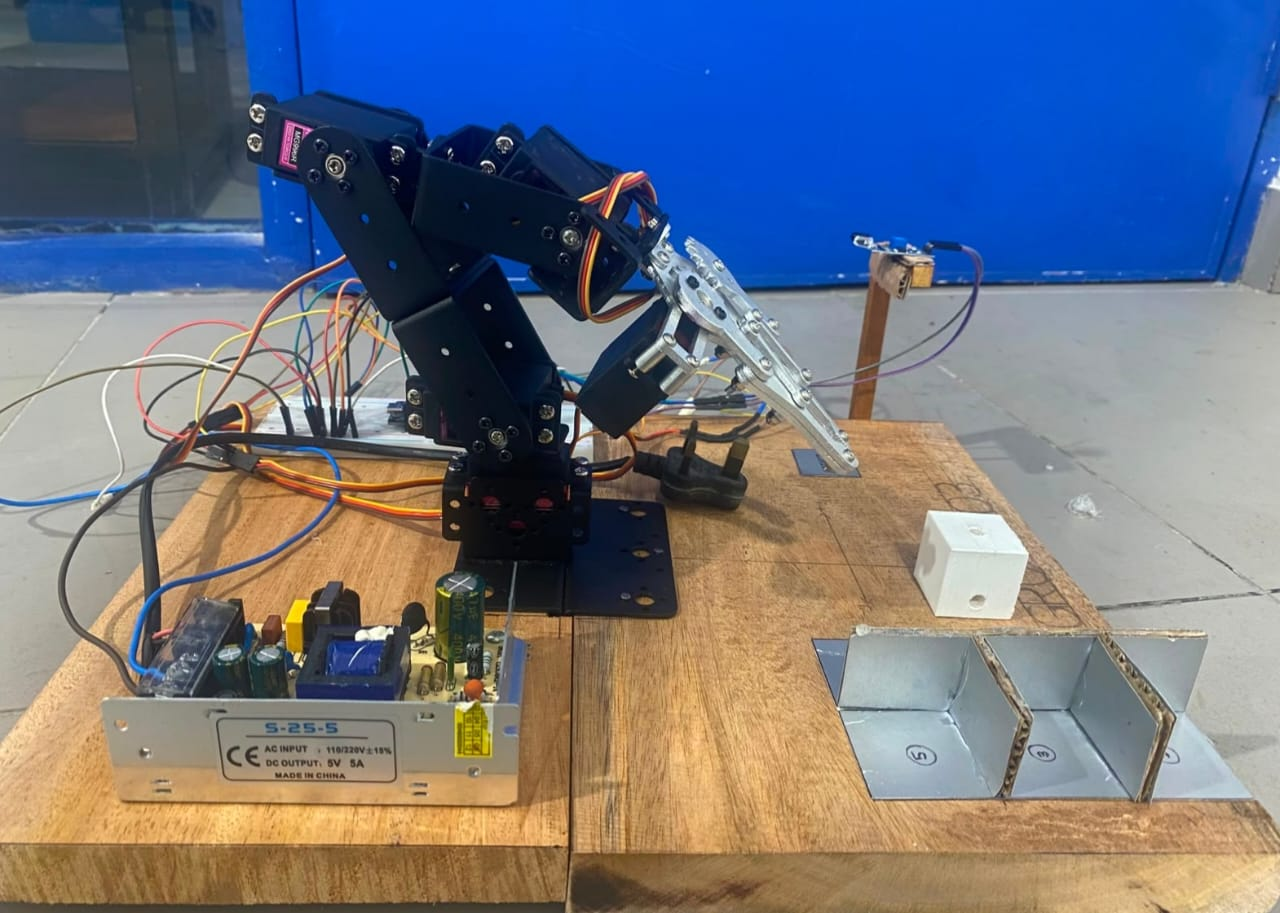
\includegraphics[width=\columnwidth]{figures/final assembly.jpeg}
    \caption{Final assembled prototype of the developed robotic arm}
    \label{fig:assembly}
\end{figure}




\section{INVERSE KINEMATICS MODEL AND ANGLE CALCULATION}

\subsection{Manipulator Description}

The arm is a serial RRRR (revolute--revolute--revolute--revolute) manipulator with four actively driven position joints and a gripper. The wrist joint ($\theta_4$) is held fixed throughout the pick-and-place process. Therefore, for the purpose of positioning the gripper tip, the wrist and gripper behave as a single rigid extension of the forearm. The angle $\theta_1$ represents the base rotation angle, $\theta_2$ represents the shoulder movement angle, and $\theta_3$ represents the elbow movement angle.

\begin{table}[htbp]
    \centering
    \caption{Joint configuration of the robotic arm}
    \label{tab:joint_configuration}
    \begin{tabular}{c l l l}
        \toprule
        Joint & Name & Motion Type & Servo \\
        \midrule
        1 & Base & Yaw about vertical axis & DS3218 \\
        2 & Shoulder & Pitch & MG996R \\
        3 & Elbow & Pitch & MG996R \\
        4 & Wrist & Pitch & MG996R \\
        -- & Gripper & Open/close & MG996R \\
        \bottomrule
    \end{tabular}
\end{table}

The main link dimensions used in the kinematic model are given in Table~\ref{tab:link_details}.

\begin{table}[htbp]
    \centering
    \caption{Link dimensions used in the kinematic model}
    \label{tab:link_details}
    \begin{tabular}{c l c}
        \toprule
        Parameter & Description & Value \\
        \midrule
        $H$ & Base to shoulder effective height & 100 mm \\
        $L_1$ & Shoulder to elbow length & 100 mm \\
        $L_2$ & Elbow to gripper tip length & 210 mm \\
        $Z$ & Object height & 40 mm \\
        \bottomrule
    \end{tabular}
\end{table}

\subsubsection{Design Decision: Neutralized Wrist}

Since the prototype has a small pick-and-place workspace and relatively short travel distances, wrist pitching is held at a fixed angle throughout the operation. This fixed angle is represented by $\beta$ for convenience. In the implemented prototype, $\beta=0^\circ$, meaning that the gripper is mounted in line with the forearm.

\begin{figure}[htbp]
    \centering
    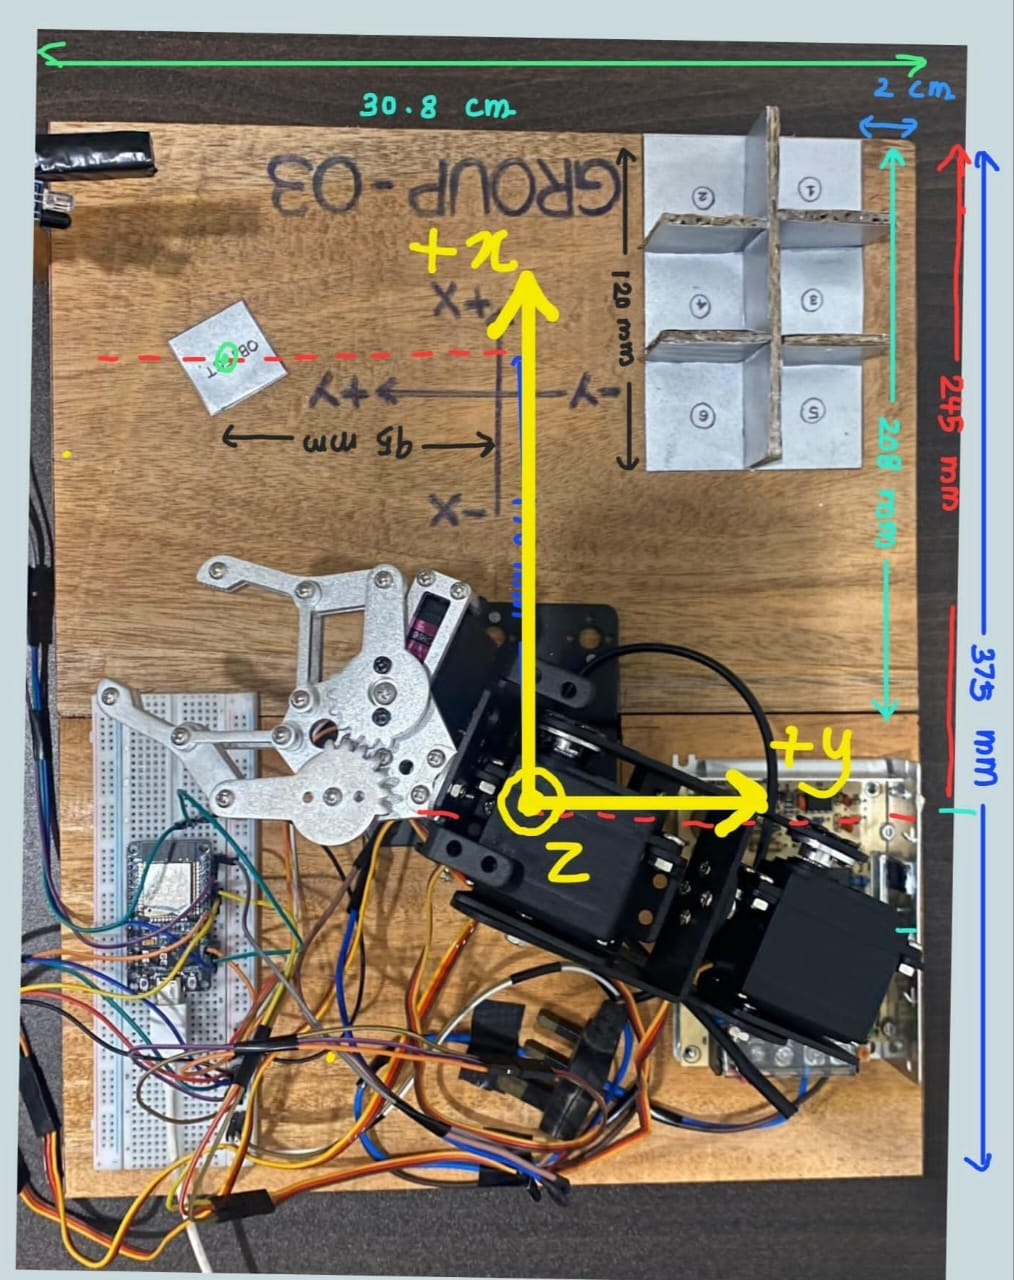
\includegraphics[width=\columnwidth]{figures/Coordinate system.jpeg}
    \caption{Coordinate system and geometric parameters of the robotic arm for inverse kinematics analysis}
    \label{fig:coordinate system}
\end{figure}

\subsubsection{Base Frame Convention}

The base frame convention matches the calibration marks on the physical workspace. The origin is located at the intersection of the base vertical rotation axis and the table surface. The $X$-axis points toward the forward workspace and placement grid, the $Y$-axis represents the lateral direction, and the $Z$-axis is vertical and positive upward.

\subsection{Denavit--Hartenberg Parameters}

The standard Denavit--Hartenberg (DH) convention is used, with the vertical axis of joint 1 and parallel horizontal pitch axes for joints 2--4. The resulting DH parameters are given in Table~\ref{tab:dh_parameters}.

\begin{table}[htbp]
    \centering
    \caption{Denavit--Hartenberg parameters}
    \label{tab:dh_parameters}
    \begin{tabular}{c c c c c}
        \toprule
        $i$ & $a_{i-1}$ & $\alpha_{i-1}$ & $d_i$ & $\theta_i$ \\
        \midrule
        1 & 0 & $0^\circ$ & $H$ & $\theta_1$ \\
        2 & 0 & $90^\circ$ & 0 & $\theta_2$ \\
        3 & $L_1$ & $0^\circ$ & 0 & $\theta_3$ \\
        4 & $L_2$ & $0^\circ$ & 0 & $\theta_4=\beta$ \\
        5 (tool) & $L_g$ & $0^\circ$ & 0 & 0 \\
        \bottomrule
    \end{tabular}
\end{table}

\subsection{Explicit Joint Transformation Matrices}

Using the standard DH convention, the transformation matrix for each joint is expressed as

\begin{equation}
{}^{i-1}A_i =
\begin{bmatrix}
\cos\theta_i &
-\sin\theta_i &
0 &
a_{i-1}
\\
\sin\theta_i\cos\alpha_{i-1} &
\cos\theta_i\cos\alpha_{i-1} &
-\sin\alpha_{i-1} &
-\sin\alpha_{i-1}d_i
\\
\sin\theta_i\sin\alpha_{i-1} &
\cos\theta_i\sin\alpha_{i-1} &
\cos\alpha_{i-1} &
\cos\alpha_{i-1}d_i
\\
0 & 0 & 0 & 1
\end{bmatrix}.
\label{eq:dh_general}
\end{equation}

Substituting the corresponding fixed values of $\alpha_{i-1}$ into the standard DH transformation gives the following explicit transformation matrices.

\subsubsection{Joint 1 -- Base Yaw}

For $\alpha_0=0^\circ$ and $d_1=H$,

\begin{equation}
{}^0A_1 =
\begin{bmatrix}
\cos\theta_1 & -\sin\theta_1 & 0 & 0\\
\sin\theta_1 & \cos\theta_1 & 0 & 0\\
0 & 0 & 1 & H\\
0 & 0 & 0 & 1
\end{bmatrix}.
\label{eq:a1}
\end{equation}

\subsubsection{Joint 2 -- Shoulder Pitch}

For $\alpha_1=90^\circ$ and $a_1=0$,

\begin{equation}
{}^1A_2 =
\begin{bmatrix}
\cos\theta_2 & 0 & \sin\theta_2 & 0\\
\sin\theta_2 & 0 & -\cos\theta_2 & 0\\
0 & 1 & 0 & 0\\
0 & 0 & 0 & 1
\end{bmatrix}.
\label{eq:a2}
\end{equation}

\subsubsection{Joint 3 -- Elbow Pitch}

For $\alpha_2=0^\circ$ and $a_2=L_1$,

\begin{equation}
{}^2A_3 =
\begin{bmatrix}
\cos\theta_3 & -\sin\theta_3 & 0 & L_1\cos\theta_3\\
\sin\theta_3 & \cos\theta_3 & 0 & L_1\sin\theta_3\\
0 & 0 & 1 & 0\\
0 & 0 & 0 & 1
\end{bmatrix}.
\label{eq:a3}
\end{equation}

\subsubsection{Joint 4 -- Wrist Pitch}

The wrist joint is fixed at $\theta_4=\beta$. Therefore, for $\alpha_3=0^\circ$ and $a_3=L_2$,

\begin{equation}
{}^3A_4 =
\begin{bmatrix}
\cos\beta & -\sin\beta & 0 & L_2\cos\beta\\
\sin\beta & \cos\beta & 0 & L_2\sin\beta\\
0 & 0 & 1 & 0\\
0 & 0 & 0 & 1
\end{bmatrix}.
\label{eq:a4}
\end{equation}

The transformation from the base frame to the wrist frame is therefore

\begin{equation}
{}^0A_4 =
{}^0A_1
{}^1A_2
{}^2A_3
{}^3A_4.
\label{eq:a04}
\end{equation}

Since $\theta_4$ is fixed at the constant value $\beta$, the transformation contains only three unknown joint variables, namely $\theta_1$, $\theta_2$, and $\theta_3$. These variables can be determined from the desired gripper-tip position $(X,Y,Z)$ without performing a separate wrist-orientation decoupling step.

\subsection{Forward Kinematics}

Multiplying the transformation chain, the gripper-tip position in the base frame can be expressed using the cumulative pitch angle

\begin{equation}
\phi = \theta_2+\theta_3+\theta_4.
\label{eq:phi}
\end{equation}

The radial distance from the base axis is

\begin{equation}
r =
L_1\cos(\theta_2)
+
L_2\cos(\theta_2+\theta_3)
+
L_g\cos(\phi).
\label{eq:radial}
\end{equation}

The relative vertical displacement from the shoulder axis is

\begin{equation}
z_{\mathrm{rel}} =
L_1\sin(\theta_2)
+
L_2\sin(\theta_2+\theta_3)
+
L_g\sin(\phi).
\label{eq:zrel}
\end{equation}

Therefore, the Cartesian coordinates of the gripper tip are

\begin{align}
X &= r\cos(\theta_1), \label{eq:x_position}\\
Y &= r\sin(\theta_1), \label{eq:y_position}\\
Z &= H+z_{\mathrm{rel}}. \label{eq:z_position}
\end{align}

\subsection{Reduction Under the Neutral Wrist Assumption}

Since $\theta_4$ is held at the fixed constant $\beta$, the effective forearm length used throughout the inverse kinematics derivation is

\begin{equation}
L_2 = 10+11 = 21~\mathrm{cm},
\qquad \beta=0^\circ.
\label{eq:effective_l2}
\end{equation}

With $\beta=0^\circ$, the gripper is collinear with the forearm, allowing the wrist and gripper extension to be treated as a rigid link for position calculation.

\subsection{Inverse Kinematics (Closed Form, Elbow-Up)}

Given a target gripper-tip position $(X,Y,Z)$ in the base frame, the horizontal radial distance is calculated as

\begin{equation}
r = \sqrt{X^2+Y^2}.
\label{eq:ik_r}
\end{equation}

The base rotation angle is obtained using the two-argument arctangent function:

\begin{equation}
\theta_1 = \operatorname{atan2}(X,Y).
\label{eq:ik_theta1}
\end{equation}

The relative vertical position with respect to the shoulder is

\begin{equation}
z_{\mathrm{rel}} = Z-H.
\label{eq:ik_zrel}
\end{equation}

The distance from the shoulder joint to the target position is

\begin{equation}
D = \sqrt{r^2+z_{\mathrm{rel}}^2}.
\label{eq:ik_d}
\end{equation}

The target position is reachable only when

\begin{equation}
|L_1-L_2| \leq D \leq L_1+L_2.
\label{eq:reachability}
\end{equation}

For the dimensions used in this prototype,

\begin{equation}
11~\mathrm{cm} \leq D \leq 31~\mathrm{cm}.
\label{eq:reachability_values}
\end{equation}

Using the law of cosines, the elbow angle is obtained from

\begin{equation}
\cos\theta_3 =
\frac{D^2-L_1^2-L_2^2}
{2L_1L_2}.
\label{eq:cos_theta3}
\end{equation}

For the selected elbow configuration,

\begin{equation}
\theta_3 =
-\cos^{-1}(\cos\theta_3).
\label{eq:theta3}
\end{equation}

The shoulder angle is then calculated as

\begin{equation}
\theta_2 =
\operatorname{atan2}(z_{\mathrm{rel}},r)
-
\operatorname{atan2}
\left(
L_2\sin\theta_3,
L_1+L_2\cos\theta_3
\right).
\label{eq:theta2}
\end{equation}

Finally, the wrist angle remains fixed at

\begin{equation}
\theta_4=\beta.
\label{eq:theta4}
\end{equation}

\subsection{Worked Example -- Picking Position}

The picking position was measured from the base rotation point as

\begin{equation}
X=-9.5~\mathrm{cm},
\qquad
Y=17~\mathrm{cm},
\qquad
Z=4~\mathrm{cm}.
\end{equation}

The radial distance is

\begin{align}
r
&= \sqrt{(-9.5)^2+17^2}\\
&=19.474~\mathrm{cm}.
\end{align}

The base angle is

\begin{align}
\theta_1
&=\operatorname{atan2}(-9.5,17)\\
&=-29.197^\circ.
\end{align}

The negative value indicates that the target is located to the left of the reference direction.

The relative vertical position is

\begin{equation}
z_{\mathrm{rel}}=4-10=-6~\mathrm{cm}.
\end{equation}

Therefore,

\begin{align}
D
&=\sqrt{19.474^2+(-6)^2}\\
&=20.378~\mathrm{cm}.
\end{align}

The elbow angle is calculated using

\begin{align}
\cos\theta_3
&=
\frac{20.378^2-10^2-21^2}
{2(10)(21)}\\
&=-0.2994.
\end{align}

Thus,

\begin{equation}
\theta_3
=
-\cos^{-1}(-0.2994)
=
-107.422^\circ.
\end{equation}

The shoulder angle is obtained from

\begin{equation}
\theta_2 =
\operatorname{atan2}(-6,19.474)
-
\operatorname{atan2}
\left(
21\sin(107.422^\circ),
10+21\cos(107.422^\circ)
\right),
\end{equation}

giving

\begin{equation}
\theta_2=62.379^\circ.
\end{equation}

Therefore, the geometric joint angles at the pick position are approximately

\begin{equation}
\boxed{
\theta_1=-29.2^\circ,\quad
\theta_2=62.4^\circ,\quad
|\theta_3|=107.4^\circ
}
\end{equation}

\subsection{Why Calibrated Servo Angles Were Used Instead of Real-Time IK}

The inverse kinematics calculation described above was performed for all seven target positions, including the picking position and six placing positions. The resulting angles were used as an initial reference for testing the robotic arm. Although the calculated values were close to the required positions, physical calibration was required to obtain accurate servo angles.

A calibration program was therefore used to manually adjust the servo positions for each target location. The final calibrated angles were then hardcoded directly into the firmware. Therefore, both the mathematical inverse kinematics model and the physical calibration process were used to obtain the final joint-angle values.

The use of calibrated angles is suitable for this prototype for the following reasons:

\begin{itemize}
    \item The workspace is relatively small, and the angular variation between one placing slot and another is limited.
    
    \item Since all target positions are fixed, the joint angles do not need to be recalculated during every execution. The calibrated values can instead be stored directly in the firmware, reducing unnecessary ESP32 processing.
    
    \item Using calibrated servo angles reduces the possibility of commanding the robotic arm toward an unreachable position.
    
    \item The servo angles can be manually adjusted according to the actual mechanical configuration of the robotic arm rather than relying only on the ideal mathematical model.
    
    \item Since computer vision is not used for determining the target positions at this stage, repeated real-time inverse kinematics calculations are not required for the fixed target positions.
\end{itemize}

\subsection{Comparison of Calculated Angles with Calibrated Servo Values}

The same inverse kinematics procedure used for the picking position was repeated for each of the six storage slots using their measured $(X,Y)$ coordinates and the same vertical displacement. The calibrated picking position was used as the reference point.

The fixed offsets obtained during calibration were used to convert the calculated geometric joint angles into corresponding servo values. The offsets were

\begin{align}
K &= 60.803^\circ && \text{(base)},\\
c_1 &= 60.803^\circ && \text{(shoulder)},\\
c_2 &= 60.803^\circ && \text{(elbow)}.
\end{align}

These offset values were kept unchanged for all six storage slots. The calculated joint angles and the corresponding calibrated servo values are summarized in Table~\ref{tab:angle_comparison}.

\begin{table*}[htbp]
    \centering
    \caption{Comparison between calculated joint angles and calibrated servo values}
    \label{tab:angle_comparison}
    \begin{tabular}{c c c c c c c}
        \toprule
        Position &
        $\theta_1$ Calculated &
        $\theta_2$ Calculated &
        $\theta_3$ Calculated &
        Base: Calc./Code &
        Shoulder: Calc./Code &
        Elbow: Calc./Code \\
        \midrule
        Pick  & $-29.2^\circ$ & $62.4^\circ$ & $107.4^\circ$ & $90.0^\circ/90^\circ$ & $45.0^\circ/45^\circ$ & $95.0^\circ/95^\circ$ \\
        Slot 1 & $27.1^\circ$ & $36.7^\circ$ & $71.5^\circ$ & $33.7^\circ/38^\circ$ & $19.3^\circ/30^\circ$ & $59.0^\circ/67^\circ$ \\
        Slot 2 & $18.4^\circ$ & $44.0^\circ$ & $82.1^\circ$ & $42.4^\circ/45^\circ$ & $26.7^\circ/40^\circ$ & $69.7^\circ/80^\circ$ \\
        Slot 3 & $31.9^\circ$ & $52.6^\circ$ & $94.2^\circ$ & $28.9^\circ/30^\circ$ & $35.2^\circ/40^\circ$ & $81.7^\circ/85^\circ$ \\
        Slot 4 & $22.1^\circ$ & $60.3^\circ$ & $104.7^\circ$ & $38.7^\circ/40^\circ$ & $42.9^\circ/50^\circ$ & $92.3^\circ/100^\circ$ \\
        Slot 5 & $38.4^\circ$ & $66.5^\circ$ & $112.8^\circ$ & $22.4^\circ/25^\circ$ & $49.1^\circ/55^\circ$ & $100.3^\circ/105^\circ$ \\
        Slot 6 & $27.3^\circ$ & $76.2^\circ$ & $124.6^\circ$ & $33.5^\circ/35^\circ$ & $58.8^\circ/55^\circ$ & $112.2^\circ/109^\circ$ \\
        \bottomrule
    \end{tabular}
\end{table*}

\subsubsection{Discussion of Results}

The difference between the calculated and calibrated base angles is approximately $1^\circ$--$4^\circ$ for the target positions. The close agreement indicates that the horizontal geometry, link lengths, and base rotation direction used in the model are consistent with the physical configuration. The base angle primarily depends on the horizontal position of the target and is independent of the object height.

The shoulder ($\theta_2$) and elbow ($\theta_3$) angles exhibit larger differences, approximately $3^\circ$--$16^\circ$, for the storage slots. These differences can be attributed mainly to practical mechanical and measurement factors rather than to the inverse kinematics formulation itself. The main contributing factors include:

\begin{itemize}
    \item The slot coordinates were measured manually from the physical workspace, which can introduce small measurement errors.
    
    \item The actual link dimensions can differ slightly from the ideal model because of bracket thickness, servo-horn offsets, and mounting tolerances.
    
    \item The mathematical model assumes that the gripper is exactly aligned with the forearm. In practice, a small wrist or gripper offset may exist and can affect the calculated joint angles.
\end{itemize}

Accordingly, the differences between the calculated geometric angles and the calibrated servo values are mainly associated with real-world mechanical tolerances, measurement uncertainties, and the difference between the idealized kinematic model and the physical robotic arm.
\cite{hayat2015robot}

\section{ELECTRONIC SYSTEM AND MICROCONTROLLER IMPLEMENTATION}

\subsection{Hardware Components}

The electronic system of the 5-DOF pick-and-place robotic arm consists of a microcontroller unit, servo motors, an object detection sensor, and a dedicated power supply system. The hardware components were selected to provide sufficient torque, accurate joint movement, and reliable control during the automated pick-and-place operation.

The entire system receives input on the target location, controls the robotic arm's movements through servo motors, detects the presence of an object using an IR sensor, and then executes the required sequence of gripping and placement. The primary aim of the electronic system is to translate the calculated joint angles of the inverse kinematics algorithm into physical motion of the robotic arm.

\subsubsection{ESP32 Microcontroller}

The ESP32 development board was selected as the main controller due to its processing capability, multiple GPIO pins, PWM output support, and compatibility with servo motor control applications.

The ESP32 performs the following tasks:

\begin{itemize}
    \item Generates PWM signals required for servo motor control.
    \item Receives input signals from the IR sensor.
    \item Executes the pick-and-place control algorithm.
    \item Stores and processes the calculated servo angle values.
    \item Coordinates the movement of all five servo motors.
\end{itemize}

The ESP32 acts as the communication bridge between the mathematical model and the physical robotic system. The calculated inverse kinematics results are converted into servo commands and transmitted through PWM control signals.

\subsubsection{Servo Motors}

The robotic arm uses five servo motors to provide five degrees of freedom. According to the system design, each joint performs a specific function, as shown in Table~\ref{tab:servo_configuration}.

\begin{table}[htbp]
\centering
\caption{Servo Motor Configuration}
\label{tab:servo_configuration}
\begin{tabular}{lll}
\toprule
\textbf{Joint} & \textbf{Function} & \textbf{Servo Motor} \\
\midrule
Joint 01 & Base rotation & DS3218 \\
Joint 02 & Shoulder movement & MG996R \\
Joint 03 & Elbow movement & MG996R \\
Joint 04 & Wrist movement & MG996R \\
Joint 05 & Gripper movement & MG996R \\
\bottomrule
\end{tabular}
\end{table}

The DS3218 servo motor was used for the base rotation due to its higher torque requirement. The MG996R servo motors were used for the remaining joints because they provide adequate torque and are commonly used for robotic arm applications.

The servo motors receive angular position commands from the ESP32 and rotate to the required positions calculated through the inverse kinematics algorithm.

\subsubsection{IR Object Detection Sensor}

An infrared (IR) sensor was integrated into the system to detect the presence of objects before starting the pick operation.

The sensor performs the following functions:

\begin{itemize}
    \item Detects whether an object is available for pickup.
    \item Provides a trigger signal to the ESP32.
    \item Prevents unnecessary movement when no object is detected.
\end{itemize}

When the IR sensor detects an object, the ESP32 executes the pick-and-place sequence.

\subsubsection{Power Supply System}

Since multiple servo motors require high current during movement, an external power supply was used instead of directly powering the motors from the ESP32.

The power system consists of:

\begin{itemize}
    \item 5~V external SMPS power supply.
    \item Breadboard-based power distribution.
    \item Separate servo power connections.
\end{itemize}

The external power supply improves system stability by reducing voltage drops and preventing controller resets caused by high servo current consumption. The project cost breakdown identifies the use of a 5~V/5~A SMPS power supply for the servo system.


\subsection{ESP32 Control Implementation}

\subsubsection{Servo Library Implementation}

The ESP32 program was developed using the Arduino IDE environment. The servo control system uses a servo library to generate PWM signals for controlling the angular position of each motor.

Each servo motor is assigned:

\begin{itemize}
    \item A specific GPIO pin.
    \item An initial position.
    \item A target angle.
    \item A movement sequence.
\end{itemize}

The program structure consists of:

\begin{enumerate}
    \item Servo initialization.
    \item Sensor initialization.
    \item Position definition.
    \item Movement functions.
    \item Pick-and-place sequence execution.
\end{enumerate}

\subsubsection{PWM-Based Servo Control}

Servo motors are controlled using Pulse Width Modulation (PWM). The relationship between the PWM signal and servo angle is based on the following principles:

\begin{itemize}
    \item A specific pulse width corresponds to a specific angular position.
    \item Changing the PWM signal changes the servo position.
\end{itemize}

The ESP32 generates PWM signals according to the required joint angles. The overall conversion process is illustrated in Fig.~\ref{fig:ik_servo_flow}.

\begin{figure}[htbp]
\centering
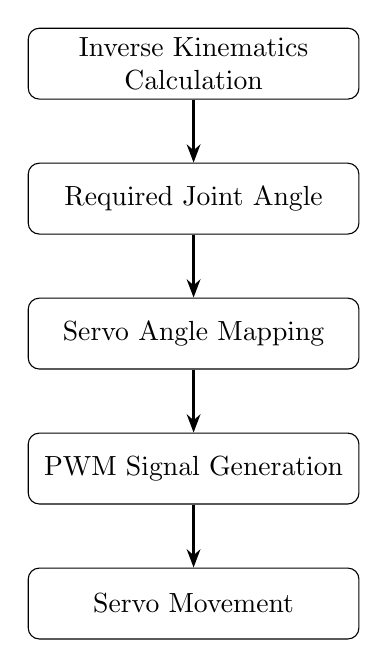
\begin{tikzpicture}[
    node distance=8mm,
    box/.style={
        rectangle,
        draw,
        rounded corners,
        minimum width=42mm,
        minimum height=9mm,
        align=center
    },
    arrow/.style={-{Stealth},thick}
]

\node[box] (ik) {Inverse Kinematics\\Calculation};
\node[box, below=of ik] (angle) {Required Joint Angle};
\node[box, below=of angle] (mapping) {Servo Angle Mapping};
\node[box, below=of mapping] (pwm) {PWM Signal Generation};
\node[box, below=of pwm] (movement) {Servo Movement};

\draw[arrow] (ik) -- (angle);
\draw[arrow] (angle) -- (mapping);
\draw[arrow] (mapping) -- (pwm);
\draw[arrow] (pwm) -- (movement);

\end{tikzpicture}
\caption{Conversion of inverse kinematics results into servo movement}
\label{fig:ik_servo_flow}
\end{figure}

The calculated angles are adjusted according to the mechanical offset of each servo and converted into suitable PWM commands.

\subsubsection{Software Structure}

The control program was developed using the Arduino IDE environment. The software was organized into different functional sections to simplify system operation and debugging. The main program structure consists of initialization, movement control functions, and the main control loop.

\paragraph{Initialization Section:}
During system initialization:

\begin{itemize}
    \item Servo motors are connected to the assigned ESP32 pins.
    \item Initial joint positions are defined.
    \item The IR sensor input is configured.
    \item The robotic arm is moved to the home position.
\end{itemize}

\paragraph{Movement Control Functions:}
Separate functions were developed for:

\begin{itemize}
    \item Moving the arm to the pickup position.
    \item Controlling the gripper operation.
    \item Moving to the storage positions.
    \item Returning the arm to the initial position.
\end{itemize}

\paragraph{Main Control Loop:}
The main loop continuously monitors the IR sensor status. When an object is detected, the ESP32 executes the programmed pick-and-place sequence.


\subsection{Pick-and-Place Control Algorithm}

The developed robotic arm follows a predefined automated sequence to perform object handling. The system receives a target coordinate, calculates the required joint positions, moves the arm to the required location, picks the object using the gripper, and places it into the assigned position. The operation is repeated for multiple positions within the storage box.

The complete operation consists of the following steps:

\subsubsection{System Initialization}

When the system is powered on, the ESP32 initializes all connected components. The servo motors move to their predefined home positions to establish a reference starting point. The initialization process ensures that the robotic arm begins every operation from a known configuration.

\subsubsection{Object Detection}

The IR sensor continuously monitors the workspace for object presence. When an object is detected:

\begin{enumerate}
    \item The sensor sends a signal to the ESP32.
    \item The controller processes the input.
    \item The pick operation is initiated.
\end{enumerate}

\subsubsection{Movement to Pick Position}

The desired object position is converted into joint angles using the inverse kinematics algorithm. The ESP32 then sends the calculated angles to the servo motors, causing the robotic arm to move through coordinated joint movements.

The movement involves:

\begin{itemize}
    \item Base rotation adjustment.
    \item Shoulder positioning.
    \item Elbow movement.
    \item Wrist alignment.
    \item Gripper positioning.
\end{itemize}

\subsubsection{Object Gripping}

Once the robotic arm reaches the pickup position, the gripper servo is activated. The gripper closes around the object and maintains sufficient holding force to transport it without slipping.

\subsubsection{Movement to Target Position}

After successfully gripping the object, the robotic arm moves towards the assigned storage location. The movement is controlled using predefined target coordinates and corresponding servo angles.

\subsubsection{Object Placement and Return}

At the target location, the gripper opens and releases the object into the storage box. After placement, the robotic arm returns to the home position and waits for the next object detection signal.



\section{EXPERIMENTAL RESULTS AND DISCUSSION}

\subsection{Mechanical Testing}

Mechanical testing was conducted to evaluate the stability, movement capability, and overall performance of the robotic arm structure. The main testing areas included structural stability, joint movement, and load handling capability. During development, several mechanical challenges were encountered, including arm assembly, joint alignment, load handling, and correct motor mounting.

To overcome these issues, the arm structure was reinforced, joint positions were adjusted, and a commercially available robotic arm kit was integrated as the final mechanical platform. Individual joint testing was performed to verify the following:

\begin{itemize}
    \item Smooth base rotation.
    \item Accurate shoulder and elbow movement.
    \item Proper wrist positioning.
    \item Reliable gripper operation.
\end{itemize}

Servo calibration was carried out to achieve synchronized and accurate joint movement.

\subsection{Angle Verification}

The accuracy of the inverse kinematics implementation was verified by comparing the calculated joint angles with the actual servo movements. The verification process involved the following steps:

\begin{enumerate}
    \item Providing the desired end-effector coordinates.
    \item Calculating joint angles using inverse kinematics.
    \item Sending the calculated values to the ESP32.
    \item Observing the actual servo positions.
    \item Adjusting calibration offsets where required.
\end{enumerate}

Coordinate calibration was performed through repeated testing to improve the positioning accuracy of the robotic arm. The results confirmed that the calculated angles could be successfully converted into accurate physical movements.

\subsection{Pick and Place Performance}

The complete robotic system was tested by performing multiple pick-and-place operations. The performance evaluation included object detection, gripping performance, placement accuracy, and system repeatability.

\subsubsection{Object Detection}

The IR sensor successfully detected the presence of objects and triggered the automated pick-and-place operation.

\subsubsection{Gripping Performance}

The gripper mechanism was tested to ensure reliable object handling. Modifications were made to improve gripping performance and prevent object slipping during the pick-and-place process.

\subsubsection{Placement Accuracy}

Placement accuracy was improved through the following methods:

\begin{itemize}
    \item Servo calibration.
    \item Coordinate adjustment.
    \item Repeated testing.
\end{itemize}

These adjustments helped improve the consistency of object placement at the designated positions.

\subsubsection{System Repeatability}

The robotic arm demonstrated repeatable movement by successfully completing multiple operating cycles. Software debugging and system integration testing were performed to ensure smooth communication between the ESP32, sensors, and servo motors.\cite{baby2017pick}



\section{conclusion}

This project successfully developed a 5-DOF pick-and-place robotic arm by integrating mechanical design, inverse kinematics, electronic control, and embedded programming. A conceptual mechanical structure was designed using SolidWorks to analyse the robotic arm configuration and joint arrangement. Although the initial design was developed through CAD modeling, the final prototype was implemented using a commercially available robotic arm structure to achieve reliable mechanical operation.
The inverse kinematics algorithm successfully calculated the required joint angles according to the desired end-effector positions. These calculated angles were implemented using an ESP32 microcontroller to control five servo motors and achieve coordinated robotic movement. The integration of an IR sensor enabled automated object detection, while the gripper mechanism allowed successful object handling and placement. The experimental results demonstrated that the developed system was capable of performing automated pick-and-place operations with accurate positioning and repeatable movement.


\section{FUTURE WORK}

Although the developed robotic arm successfully performs basic pick-and-place
operations, several improvements can be implemented to enhance system
intelligence, accuracy and industrial applicability.

\subsection{Camera-Based Object Recognition}

A camera-based vision system can replace the current IR-based detection method
to automatically identify the position, shape, and orientation of objects.
This would allow the robotic arm to operate with different object locations
without requiring predefined detection positions.

\subsection{AI-Based Vision System}

Artificial intelligence techniques can be incorporated into the vision system
to enhance the autonomous capabilities of the robotic arm. The proposed
AI-based system can provide the following functionalities:

\begin{itemize}
    \item \text{Object Classification:} Identifying and categorizing
    different types of objects based on their visual characteristics.

    \item \text{Real-Time Tracking:} Continuously tracking the position of
    objects during the robotic operation.

    \item \text{Autonomous Decision Making:} Selecting appropriate actions
    based on the detected object and its position.
\end{itemize}

\subsection{Feedback Control Using Encoders}

Currently, the robotic arm operates using predefined servo positions. Rotary
encoders can be incorporated into the joints to provide real-time position
feedback. This would enable closed-loop control and improve the positioning
accuracy of the robotic arm.

\subsection{Higher Payload Design}

Future improvements can include stronger mechanical structures and higher
torque actuators to increase the payload capacity of the robotic arm. This
would allow the system to handle heavier objects and expand its potential
applications.

\subsection{Wireless Monitoring and Control}

Wireless communication technologies such as Wi-Fi or Bluetooth can be
integrated into the robotic arm to enable remote monitoring and operation.
This would allow users to monitor the system status and control the robotic
arm without requiring a direct wired connection.




\section{acknowledgment}

We would like to express their sincere gratitude to Dr. Chinthaka Kumara for providing the project idea and for his valuable supervision throughout the project. Also deeply grateful to Dr. Randima Dinalankara for providing valuable guidance, technical insights and encouragement which helped us to improve our work throughout the project.

We would also like to thank the Department of Computer Engineering, Faculty of Engineering, University of Sri Jayewardenepura, for providing the facilities and resources to successfully complete this project. It was a great learning opportunity for us, allowing us to apply our theoretical knowledge to a practical engineering problem and gain valuable experience in designing, developing and testing a robotic system.



\bibliographystyle{IEEEtran}
\bibliography{references}

\end{document}

